\section{Calibration and Estimation}
\label{sec:calibration}

The model is described by a large number of parameters that govern the number of contacts a person has, the likelihood of becoming infected on each contact, the likelihood of developing light or strong symptoms or even dying from the disease as well as the duration each stage of the disease takes.

Most of these parameters can be calibrated from existing datasets or the medical literature. Only the infection probabilities have to be estimated inside the model by fitting it to time series data of case numbers and fatality rates.


\subsection{Medical Parameters}

\subsubsection{Length of Presymptomatic Stage / Incubation Period}


Estimates of the incubation period usually give a range from 2 to 12 days. A meta analysis by \cite{McAloon2020} comes to the conclusion that ``The incubation period distribution may be modelled with a lognormal distribution with pooled $\mu$ and $\sigma$ parameters (95 \% CIs) of 1.63 (95 \% CI 1.51 to 1.75) and 0.50 (95 \% CI 0.46 to 0.55), respectively.'' For simplicity we discretize this distribution into four bins.


\subsubsection{Begin of Infectiousness}

The period between infection and onset of infectiousness is called latent or latency period. However, the latency period is rarely given in epidemiological reports on Covid-19. Instead, scientists and agencies usually report the incubation period, the period from infection to the onset of symptoms. A few studies used measurements of virus shedding to estimate infectiousness during the course of the disease. When measurements started before the onset of symptoms the development of the viral load before symptoms gives us an indication of number of days between the onset of infectiousness and symptoms.

The European Centre for Disease Prevention and Control estimates that people become infectious between one and two days before the symptoms set in. This is similar to \cite{He2020} who estimate this to take 2.3 days and is in line with \cite{Peak2020}.

Given these numbers and the length of the incubation period we can calculate the latency period for symptomatic people. To our knowledge no estimates for the latency period of asymptomatic cases of COVID-19 exist. We assume it to be the same for symptomatic and asymptomatic cases.

Thus, we arrive at the following distribution for latency periods: 40\% have one day. 35\% have two days. 20\% have three days and 5\% have 5 days.


\subsection{Duration of Infectiousness}

We assume that the duration of infectiousness is the same for both symptomatic and asymptomatic individuals as evidence suggests little differences in the transmission rates of SARS-CoV-2 virus between symptomatic and asymptomatic patients (\cite{Yin2020}) and that the viral load between symptomatic and asymptomatic individuals are similar (\cite{Zou2020}, \cite{Byrne2020}, \cite{Singanayagam2020}).

Our distribution of the duration of infectiousness is based on \cite{Byrne2020}.

For symptomatic cases they arrive at 0-5 days before symptom onset (figure 2) and 3-8 days of infectiousness afterwards.\footnote{Viral loads may be detected much later but 8 days seems to be the time after which most people are culture negative, as also reported by \cite{Singanayagam2020}} Thus, we arrive at 0 to 13 days as the range for infectiousness among individuals who become symptomatic (see also figure 5). This duration range is very much in line with the meta-analysis’ reported evidence for asymptomatic individuals (see their figure 1). Thus, we arrive at 0 to 13 days as the range for infectiousness among individuals who become symptomatic. This duration range is very much in line with the meta-analysis' reported evidence for asymptomatic individuals.

Following this evidence we assume the following discretized distribution of the infectiousness period: 10\% of individuals are infectious for three days, 25\% for five days, another 25\% for seven days, 20\% for nine days and 20\% for eleven days.


\subsection{Duration of Symptoms}

We use the duration to recovery of mild and moderate cases reported by \cite[Figure~S3, Panel~2]{Bi2020} for the duration of symptoms for asymptomatic and non-ICU requiring symptomatic cases.

We collapse the data to the following distribution: 10\% recover after 15 days and 30\% require 18, 22 or 27 days respectively.

% These long symptom durations align with reports by \cite{Tenforde2020}.

These numbers are only used for mild cases. We do not disaggregate by age. Note that the length of symptoms is not very important in our model given that individuals stop being infectious before their symptoms cease.


\subsubsection{Time from Symptom Onset to Admission to ICU}

The data on how many percent of symptomatic patients will require ICU is pretty thin. We rely on data by the US CDC (\cite{Stokes2020}) and \href{https://github.com/BDI-pathogens/OpenABM-Covid19/blob/master/documentation/parameters/parameter_dictionary.md}{the OpenABM-Project (2020-09-14)}.

From these sources we arrive at the following probabilities of requiring intensive care:

\begin{table}[!ht]
    \caption{Shares of symptomatic patients who will require ICU care by age groups.}
    \label{tab:symptomatic-to-ICU}
    \centering

    \begin{tabular}{ll}
        \toprule
        Age Group & Share \\
        \midrule
        0-9 & 0.00005 \\
        10-19 & 0.00030 \\
        20-29 & 0.00075 \\
        30-39 & 0.00345 \\
        40-49 & 0.01380 \\
        50-59 & 0.03404 \\
        60-69 & 0.10138 \\
        70-79 & 0.16891 \\
        80-100 & 0.26871 \\
        \bottomrule
    \end{tabular}

\end{table}

For those who will require intensive care we follow \cite{Chen2020} who estimate the time from symptom onset to ICU admission as 8.5 $\pm$ 4 days.

This aligns well with numbers reported for the time from first symptoms to hospitalization: \cite{Gaythorpe2020} report a mean of 5.76 with a standard deviation of 4. This is also in line with the durations collected by \href{https://www.rki.de/DE/Content/InfAZ/N/Neuartiges_Coronavirus/Steckbrief.html#doc13776792bodyText16}{the Robert Koch Institut}.

We assume that the time between symptom onset and ICU takes 4, 6, 8 or 10 days with equal probabilities. These times mostly matter for the ICU capacities.


\subsubsection{Death and Recovery from ICU}

We take the survival probabilities and time to death and time until recovery from intensive care from the \href{https://tinyurl.com/y5owhyts}{OpenABM Project}.

They report time until death to have a mean of 11.74 days and a standard deviation of 8.79 days. Approximating this with the normal distribution, we have nearly 10\% probability mass below 0. We use it nevertheless as several other distributions (such as chi squared and uniform) were unable to match the variance.
Discretizing this leads to 41\% of individuals who die from Covid-19 to die after one day in intensive care. 22\% day after 12 days, 29\% after 20 days and 7\% after 32 days. Again, we rescale this for every age group among those that will not survive.

They report time until recovery to have a mean of 18.8 days and a standard deviation of 12.21 days. Approximating this with the normal distribution, we have over 5\% probability mass below 0. Discretizing this of those who recover in intensive care 22\% do so after one day, 30\% after 15 days, 28\% after 25 days and 18\% after 45 days.



\subsection{Number of Contacts}

% Mossong data
We calibrate the parameters for the predicted numbers of contacts from contact diaries of over 2000 individuals from Germany, Belgium, the Netherlands and Luxembourg \citep{Mossong2008}. Each contact diary contains all contacts an individual had throughout one day, including information on the other person (such as age and gender) and information on the contact. Importantly, for each contact individuals entered of which type the contact (school, leisure, work etc.) was and how frequent the contact with the other person is.

Thus, we can use the empirical distributions from this data as pre-pandemic number of contacts.


\subsection{Assortative Matching}

As mentioned in section \ref{sec:matching}, the probability that two individuals are matched can depend on background characteristics. In particular, we allow this probability to depend on age and county of residence. While we do not have good data on geographical assortativeness and just roughly calibrate it such that 60 \% of contacts are within the same county,\footnote{We are working on improving this estimation with mobility data.} we can calibrate the age assortativeness from the same data we use to calibrate the number of contacts.

\begin{figure}[!ht]
    \centering
    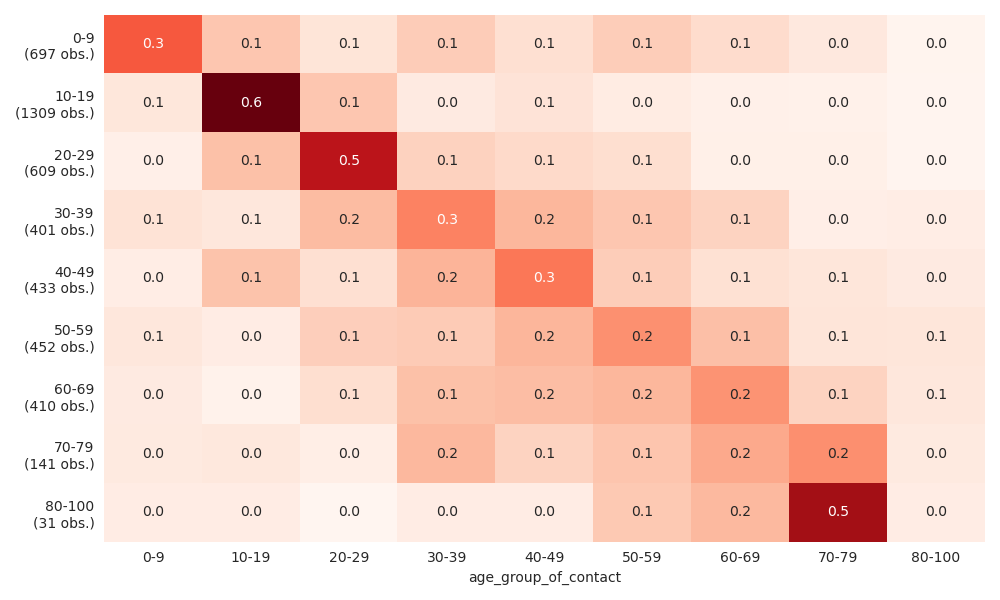
\includegraphics[width=0.7\textwidth]{../figures/assortative_matching_probability_example.png}
    \caption{Distribution of random non-work contacts by age of participants}
    \label{fig:assortativeness}
\end{figure}

Figure~\ref{fig:assortativeness} shows that overall contacts within age groups or age groups that are closer to each other are more frequent.

\subsection{Infection Probabilities}
\label{sec:estimation}

To calibrate infection probabilities outside of the model, it would be important to know the exact duration and distance of each contact type as well as virus loads. Since this is not available in any dataset, we instead estimate those parameters inside the model by minimizing the distance between simulated and observed infection rates. Since our model includes a lot of randomness, we average simulated infection rates over several model runs.

Currently, we use data for Germany from August to October (both inclusive). We do not use earlier periods to save computational time. Moreover, we would be worried that the infection probabilities have small seasonal variation that we currently cannot model. However, we plan to expand the estimation period soon.

To avoid overfitting and simplify the numerical optimization problem, we only allow for four different probabilities: 1) for contacts in schools, preschools and nurseries. 2) for work contacts. 3) for households. 4) for leisure activities.


\section{Model Validation}

We validate our model in two ways: 1) We look at the in-sample fit over the estimation period. 2) We look at the out-of-sample fit for November. The last one is a challenging test for our model because there was a strong policy change between the estimation period and November. The model convincingly passes both tests.


\subsection{In-Sample Fit}

Despite fitting only four free parameters, the in-sample fit is very good. The best fit is achieved in the largest age groups. This is so mechanically, because we weight the deviations between simulated and observed infection rates by group sizes. The worst fit is achieved for the 80 to 100 years old. The model predicts too few infections for these groups because they have very few contacts in all contact types we have included so far. We plan to address this issue soon by adding another contact type that captures all contacts in the data by \cite{Mossong2008} that we have not included so far. Moreover, we expect an improved model fit when we allow for more free parameters.


\begin{figure}[!ht]
    \centering
    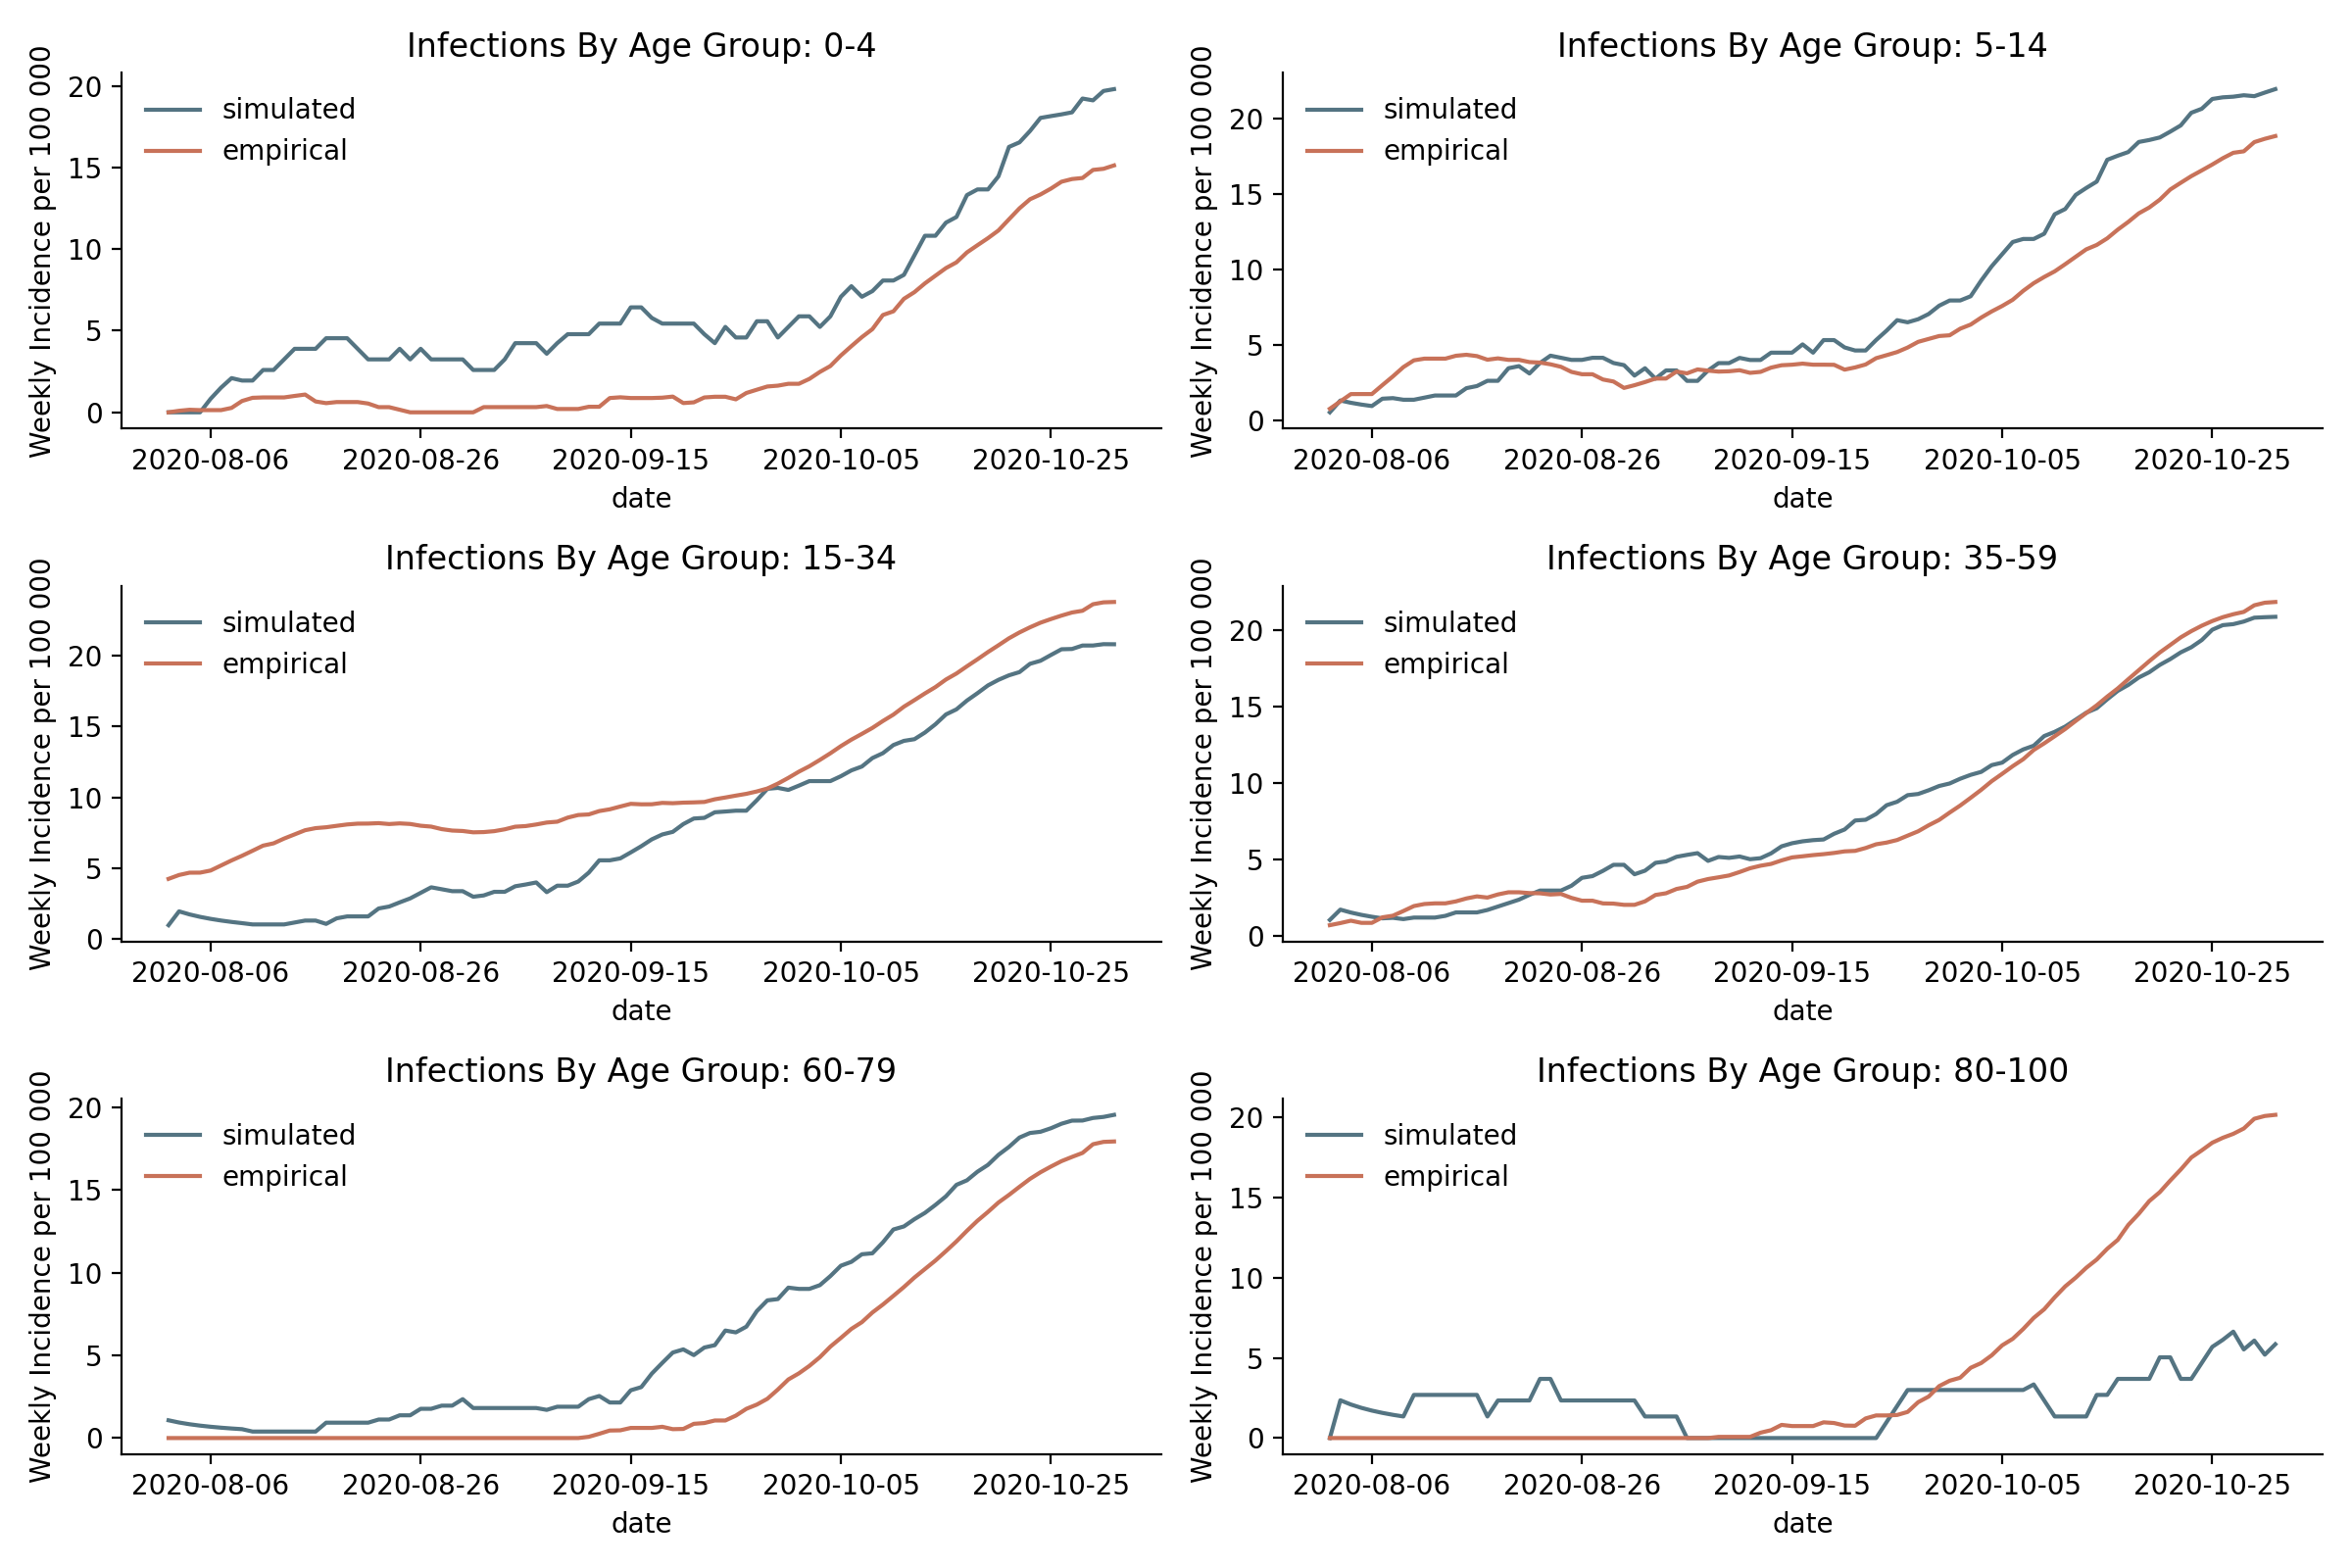
\includegraphics[width=0.7\textwidth]{../figures/goodness_of_fit_by_age_group}
    \caption{Actual vs. simulated infection and fatality rates}
    \label{fig:goodness_of_fit}
\end{figure}


\subsection{Out-of-Sample Fit}

We can assess the out-of-sample fit by projecting the effect of the lockdown light and comparing it to case numbers until now. It is important to note that this is not just a simple extrapolation of a time trend because the lockdown light only started after the estimation period. The out-of-sample fit can be assessed in Figure~\ref{fig:out-of-sample-fit}.

\begin{figure}[!ht]
    \centering
    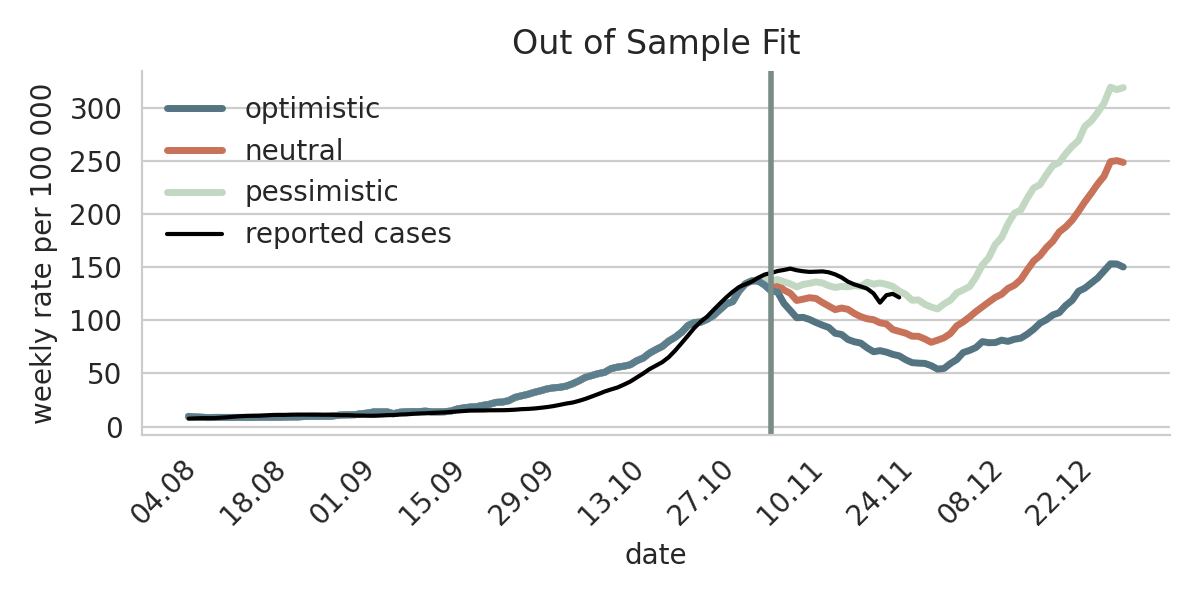
\includegraphics[width=0.7\textwidth]{../figures/out_of_sample_validation}
    \caption{Projected effect of the lockdown-light}
    \label{fig:out-of-sample-fit}
\end{figure}

The model correctly predicts the effect of the lockdown light with reasonable accuracy. In particular, the actual case numbers are between our neutral and pessimistic projection. The plot also shows that ending the lockdown light as planned on November 30 would lead to an explosive growth in case numbers in all scenarios.
